\begin{savequote}[75mm]
Nulla facilisi. In vel sem. Morbi id urna in diam dignissim feugiat. Proin molestie tortor eu velit. Aliquam erat volutpat. Nullam ultrices, diam tempus vulputate egestas, eros pede varius leo.
\qauthor{Quoteauthor Lastname}
\end{savequote}

\chapter{Basic characterizations}
% Figure:  2p_retino / cortical mag 
% Figure:  RF mapping, examples
% Figure:  RFs, aggregate/summary plots
% Figure:  GRATINGS, stimuli + example traces
% Figure:  Summary stats of OSI, DSI, "Fraction tuned"
% Figure:  RFs + ORI preferences

% Figure:  Coregistration & 2p_retino
\begin{figure}
    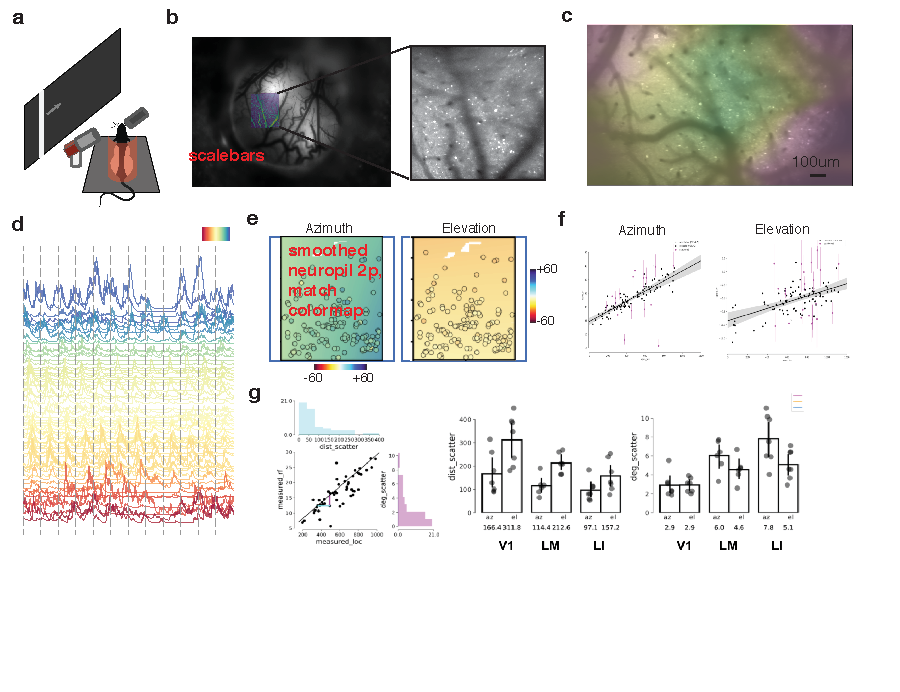
\includegraphics[width=\textwidth]{figures/chapter_2/2p_retino2.pdf}
    \vspace{.1in}
    \caption[Coregistration and area identification in 2p]{Coregistration and area identification in 2p . \textbf{a.} REFREF.
    \label{fig:2p_retino}}
\end{figure}

% Figure:  receptive_fields
\begin{figure}[t!]
    \includegraphics[width=\textwidth]{figures/chapter_3/receptive_fields.pdf}
    \vspace{.1in}
    \caption[Receptive fields]{Receptive fields. \textbf{a.} REFREF.
    \label{fig:receptive_fields}}
\end{figure}
 
\newthought{Beyond V1}, a subset of contiguous areas spanning the lateral edge of rat cortex have garnered significant attention over the past few years due to similarities between these areas in the rat and the primate ventral visual stream. Several studies \cite{Vermaercke2014, Tafazoli2017, Vinken2016NeuralCortex} have investigated these visual areas specifically in the context of visual object representations in order to test the extent to which single-unit properties characteristic of the highest levels of the primate ventral stream might also be found in the rat. These previous studies bolster the promise of the rat visual system as highly sophisticated, perhaps similar to that of primates in certain ways. 

However, monkeys and rodents differ in dramatic ways --- on one hand, similarities in how their visual systems solve a given problem are incredibly exciting, as they point to general principles conserved across specie. On the other hand, each solution is likely to be influenced by differences in the natural visual statistics by which their visual systems have been shaped. 

Despite the fact that animals with the best vision, like cats or monkeys, have been the traditional models of choice for vision studies, mice have become increasingly popular models for studying visual circuits over the past decade. This is arguably due to the immensely powerful genetic tools combined with chronic, large-scale population recordings, much of which are prohibitively challenging to use in monkeys.

In contrast, although rats have long been studied for visually-guided behaviors, large-scale cellular resolution access to their visual cortex has proved to be far more challenging. Our broad-level goal is to bridge the gap between neural circuit access and rich behavioral capacities in the rat. What has remained lacking is a basic characterization of any visual area beyond V1 in the rat. Such a systematic study provides valuable points of comparison not just with primates, but with other animal models, including mice. 

We carried out the first comprehensive survey of visual response properties across these different cortical areas in the rat. We characterize the functional organization of a subset of visual areas for the first time with cellular resolution imaging in awake, head-fixed animals. Specifically, we focused on areas V1, LM, and LI, where the most is known about single unit response properties in the rat. At a broader level, that they may be capable of supporting visual object recognition behavior is an exciting starting point for combining the powerful tools common in traditional genetic models like mice with kinds of complex behaviors associated with primates.  

% ---------------------------------------------------------------
% 2p retinotopy
% ---------------------------------------------------------------
\section{Fine-scale retinotopic organization in rat lateral cortex}
The particular region and extent of visual space that a patch of cortex represents has important implications for its function. For example, in primates, most areas of the ventral stream over-represent the central visual field, enhancing the processing of features near the fovea\cite{REFREF, Gattass2005CorticalDynamics}. Although mice, like rats, do not have foveal vision, several groups have shown consistent biases in visual field coverage in extrastriate visual areas of mice\cite{Garrett2014, Marshel2011, REFREF}. 

% 2p retinotopy -------------------------------------------------
% Retinotopic gradients + large, 2-area FOV
Using the same phase-encoding Fourier paradigm we used to map visual areas at the macroscale, we characterized retinotopic preferences across a given imaging site, as well as at the single-cell level with two-photon calcium imaging. We observed retinotopic gradients across visual axes of elevation (ventral-dorsal) and azimuth (nasal-temporal) for large FOVs ($~1mm^2$) imaged in areas V1, LM, and LI (Figure\ref{fig:2p_retino}). As a proof-of-principle, we also tested how well two visual areas could be identified within our large-FOV ($1mm$ x $2mm$) mode, and found that a clear mirror reflection was visible when parking the objective directly above an areal boundary identified by the wide-field maps. 

% Cortical magnification
To quantify how much cortex is devoted to a given unit of visual space in rat extrastriate areas, we measured cortical magnification in areas V1, LM and LI. Overall, we found that cortical magnification decreased from V1 to LM to LI, consistent with the expectation that larger areas have more cortical real estate for representing a given part of visual space (Figure\ref{fig:2p_retino}\textbf{a}). 

Cortical magnification is not necessarily isotropic, that is, along vertical (azimuth) and horizontal (elevation) axes of the visual field. For example, several studies report an expanded representation along the vertical dimension of visual space, relative to the horizontal dimension, in mouse V1\cite{Garrett2014, Liang2018, Bonin2011}.  

Similar to previous studies of mouse V1, we found an asymmetric expansion along the vertical dimension of visual space in rat V1, but also in areas LM and LI (Figure\ref{fig:2p_retino}\textbf{b}). Moreover, we found that the degree to which the vertical dimension was over-represented was significantly greater for LM and LI than for V1 (LM: p<0.05, LI: p<0.01 REFREF).

% Single-cell retinotopy / Retino scatter
While previous studies have relied on coarse retinotopy to identify the areas in which they were recording, the fine-scale retinotopic organization of cell bodies in any extrastriate area remains unknown. Single sweeps of the stimulus evoked robust responses in individual cells, and overall, cell bodies exhibited a coarse-scale retinotopic organization. However, retinotopic preferences of neighboring cells were disordered and deviated from the surrounding neuropil in V1, LM and LI (Figure\ref{fig:2p_retino}) consistent with findings in mouse visual cortex \cite{Liang2018, Andermann2011, Marques2018}. 

% Receptive fields ------------------------
In order to more finely characterize retinotopic preferences of individual cells, we quantified receptive field (RF) properties by stimulating tiled locations across the visual field (Figure\ref{fig:receptive_fields}). We mapped RFs in X\%, X\% and X\% of cells imaged in V1 (REFREF of REFREF neurons, REFREF imaging locations, REFREF rats), LM (REFREF), and LI (REFREF), respectively. Consistent with previous electrophysiology measures\cite{Vermaercke2014, Tafazoli2017}, receptive field sizes increased from V1 to LM to LI, though median sizes and relative differences were smaller than previous reports. 


The observed retinotopic scatter was ~2 fold larger for elevation than azimuth (REFREF V1: X in azimuth, X in elevation; Lm: X in azimuth, X in elevation; Li: X in azimuth, X in elevation), consistent with the observed axis differences in cortical magnification for all areas tested. The average cortical scatter in V1 ($~239.09um$), Lm ($163.48 um$), and Li ($127.17 um$) corresponded to average retinotopic displacements of  ~2.90, 5.30, and 6.45 degrees of visual angle -- roughly half or less than the average receptive field size of each visual area (REFREF, V1: ~9.49, Lm: ~10.61, LI: ~13.25 degrees of visual angle). Check, how does this compare to mouse (~20um AZ scatter and ~40um EL scatter, ~2deg)

However, at the level of individual cells, we observed no correlation between receptive field size and retinotopic scatter (Figure\ref{fig:REFREF}, stats, Pearson’s correlation, V1: corrcoef, p=X, Lm: corrcoef, p=X, Li: corrcoef, p=X).

% RFs are anisotropic, elongated along azimuth
Given the observed asymmetry in cortical magnification along azimuth and elevation (see Figure\ref{fig:2p_retino}), we calculated the angle and degree of anisotropy for each receptive field to determine whether this bias was present at the level of individual cells.

On average, receptive fields were anisotropic, with receptive field angles biased toward 0 degrees, that is, elongated along azimuth (Figure\ref{receptive_fields}). However, we did not observe a relationship between anisotropy and retinotopic scatter (REFREF, Supplemental 3.3) nor between angular bias in anisotropy (horizontally or vertically anisotropic, see Methods) and retinotopic position (REFREF, Supplemental 3.4).

% Maybe this is for better visual field coverage?
Given these observed biases in receptive field angle or anisotropy, cortical magnification, and retinotopic scatter, we wondered whether these irregularities might allow, for example, enhanced visual coverage. For all simultaneously recorded cells in a given imaging site, we compared how the distribution of receptive fields across the visual field changed if all irregularities were corrected. 

Specifically, to nullify retinotopic scatter, we assigned the predicted retinotopic position to each cell, and to nullify receptive field irregularities, we assigned size along each axis to be equal to the average of the two axes such that simulated receptive fields were perfectly isotropic ({\fig:Figure3a-b}). We calculated the variance of the distributions of RF counts across the visual field as a measure of how uniformly the receptive fields covered the visual field:  higher variance indicates RFs are clustered in select locations, while lower variance indicates RFs are evenly spread out ({\fig:Figure3c}). Overall, simulated RF distributions resulted in less uniform visual field coverage than measured RF distributions (paired test REFREF, {\fig:Figure3d} ). The fold-change in variance was greater than 1 (no difference) for X imaging sites ({\fig:Figure3e}, REFREF STATS).  


\section{Orientation and direction tuning}
Since we did not observe retinotopic organization at the REFREF um scale, we asked whether neurons might be organized by tuning to other visual features. We measured calcium responses to drifting gratings of a range of directions, spatial frequencies, speeds, and sizes (see Methods). 

Visually responsive cells were classified as responsive to a given direction of motion (direction-selective, DS), or to opposing directions of motion along a given axis (axis-selective, AS), or neither direction- or axis-selective. Overall, we found a decreasing fraction of tuned cells across the areas tested {\fig:Figure}. Splitting direction- and axis-selective cells by visual area revealed that this decrease was largely due to a decrease in the fraction of axis-selective (FIGURE). In contrast, the fraction of direction-selective neurons was not significantly different between areas (STATS).   

On average, the fraction of cells tuned for direction or orientation decreased from V1 to Li ({\fig:Figure4c}, REFREF, stats). This decrease in gratings tuning was largely driven by fewer axis-selective cells in Li ({\fig:Figure4d}, REFREF, stats). 

V1 prefers horizontally-oriented gratings (either direction). L/Lm don’t show this bias as much (what’s the right test here). REFREF


To measure the similarity in tuning between cells, we created an average tuning profile for each cell, defined as the trial-averaged response to each condition, and measured similarity as the correlation coefficient between tuning profiles (Methods). The cortical distance between cells was defined as the distance between each cell’s center of mass in the image plane. 

If visual areas exhibit a purely salt-and-pepper organization, tuning similarity and cortical distance should be statistically independent. However, we found a decrease in tuning similarity as a function of distance (REFREF, Pearons’s correlation coefficient, r=X (V1, p=#; Lm, p=#; Li=p=#)). Fit the curves with exponential or linear functions. 

Signal correlations vs. %-overlap?.
Other standard measures, for ex., broadness/sharpness?







\section{Lateral visual cortex exhibits many of the same core properties found in primates}

Since we have demonstrated the key prerequisite of establishing the behavioral ability of rats to perform visual recognition has been established, we next turned our attention to the neuronal substrates of these abilities.  Primate visual cortex is arranged hierarchically, with visual inputs from the thalamus first arriving in so-called ``striate'' cortex (also known as area V1), before being processed and forwarded through a successive chain of hierarchically-organized visual areas (area V2 > area V4 > inferotemporal cortex) curving along the ventral surface of the brain.  

Several key trends have been observed in the response properties of visual neurons as one progresses from ``lower'' to ``higher'' visual areas along this ventral pathway. First, the region of visual space that a given cell responds to (the ``receptive field'') gradually increases as one moves along the ventral pathway, with receptive fields in the highest stages of visual cortex sometimes responding to up to half of the visual field \cite{op2000spatial}. Meanwhile, selectivity for complex object features also increases along the ventral visual pathway, with neurons in later stages of the pathway responding only to very particular configurations of features \cite{Desimone1984, Logothetis1996}.  Critically, as one progresses along the ventral pathway, neurons also exhibit greater tolerance to identity-preserving transformation of the retinal image -- that is, neurons tend to retain their selectivity for particular object features even if those features are, for instance, moved around on the retina, or scaled up or down in size \cite{Ito1995}.These combined features of selectivity and tolerance are in many ways the key computational hallmarks of high-level vision \cite{DiCarlo2007, DiCarlo2012}. 

Anatomical studies have shown that the connectivity of rodent visual cortex observes a similar hierarchical pattern, with thalamic inputs arriving in an analogous striate area V1 in posterior of the brain, and then projecting ventrally to a series of interconnected extrastriate areas  \cite{Coogan1993, ETC}.  However, while these areas have been characterized anatomically, very little is known about their function.

